\section*{Titre de niveau 1}\label{titre-de-niveau-1}
\addcontentsline{toc}{section}{Titre de niveau 1}

Note: Le \{-\} dans le fichier .md signal que la section ne sera pas
numérotée.

\subsection*{Titre de niveau 2}\label{titre-de-niveau-2}
\addcontentsline{toc}{subsection}{Titre de niveau 2}

\section{Quelques rappels sur Makdown et
Pandoc}\label{quelques-rappels-sur-makdown-et-pandoc}

Pour la synthaxe, ci-dessous est présenté ``l'essentiel'' pour la
rédaction d'un document tel qu'une thèse. Pour avoir des informations
plus exhaustives et pour bien comprendre ce qu'est Markdown, voir la
\href{http://spec.commonmark.org/0.25/}{dernière spécifcation de Common
Mark}.

Pour convertir le fichier Markdown (md) en un autre fichier j'utilise le
converteur universel \href{http://pandoc.org}{Pandoc}.

\section*{Synthaxe Pandoc Markdown}\label{synthaxe-pandoc-markdown}
\addcontentsline{toc}{section}{Synthaxe Pandoc Markdown}

\subsection*{Simple mises en forme}\label{simple-mises-en-forme}
\addcontentsline{toc}{subsection}{Simple mises en forme}

Écrire en \textbf{gras} utiliser un ``\textbackslash{}emph'':
\emph{emph} (en français c'est souligner en anglais c'est en italic).
Utiliser un \textsuperscript{exposant}. Utiliser un
\textsubscript{indice} on peut même \sout{barrer}. Pour faire une
énumération (hyphenation)~:

\begin{itemize}
\tightlist
\item
  cool
\item
  cool2
\end{itemize}

une liste numérotée~:

\begin{enumerate}
\def\labelenumi{\arabic{enumi}.}
\tightlist
\item
  cool
\item
  cool2
\end{enumerate}

\subsection{Note de bas de page et
hyperlien}\label{note-de-bas-de-page-et-hyperlien}

Une note de bas de page\footnote{Ici, mettre le texte de la note de bas
  de page.}. Une lien internet {[}nom du lien{]}(adresse su lien), ex:
\href{http://pandoc.org}{Pandoc}.

\subsection*{Citations}\label{citations}
\addcontentsline{toc}{subsection}{Citations}

Pour les citation courtes en anglais les guillemets anglais ``That's one
small step for man, one giant leap for mankind''. Pour les français, le
mieux utilser les code HTML: « Vive le Québec libre ! »

Pour faire une citation plus longuqe, il suffit d'utiliser
`\textgreater{}' citation de plus de 2 lignes:

\begin{quote}
Lorem ipsum dolor sit amet, consectetur adipisicing elit, sed do eiusmod
tempor incididunt ut labore et dolore magna aliqua. Ut enim ad minim
veniam, quis nostrud exercitation ullamco laboris nisi ut aliquip ex ea
commodo consequat. Duis aute irure dolor in reprehenderit in voluptate
velit esse cillum dolore eu fugiat nulla pariatur. Excepteur sint
occaecat cupidatat non proident, sunt in culpa qui officia deserunt
mollit anim id est laborum.
\end{quote}

\subsection*{Symboles mathématques et
équations}\label{symboles-mathuxe9matques-et-uxe9quations}
\addcontentsline{toc}{subsection}{Symboles mathématques et équations}

\subsubsection*{En ligne}\label{en-ligne}
\addcontentsline{toc}{subsubsection}{En ligne}

\$votre equation\$ Après il faut connaître les symboles latex. Il y a
plein de référence en ligne, par exemple sur
\href{https://en.wikibooks.org/wiki/LaTeX/Mathematics}{Wikilivres}

Exemple: \(\overline{x}\), \(\mathcal{N}\)

\subsubsection*{Équations}\label{uxe9quations}
\addcontentsline{toc}{subsubsection}{Équations}

Utiliser \$\$votre equation\$\$ Pour faire des références, j'utilise un
filtre pandoc (écrit en python)
\href{https://github.com/tomduck/pandoc-eqnos}{Pandoc-eqnos}

\begin{equation}\prod_{i=1}^nu_n=1\label{eq:intr_1}\end{equation}

Voila une ref à l'équation \ref{eq:intr_1}

\subsection*{Figures}\label{figures}
\addcontentsline{toc}{subsection}{Figures}

Pour insérer une !{[}la légende{]}(chemin vers la figure)

\begin{figure}[htbp]
\centering
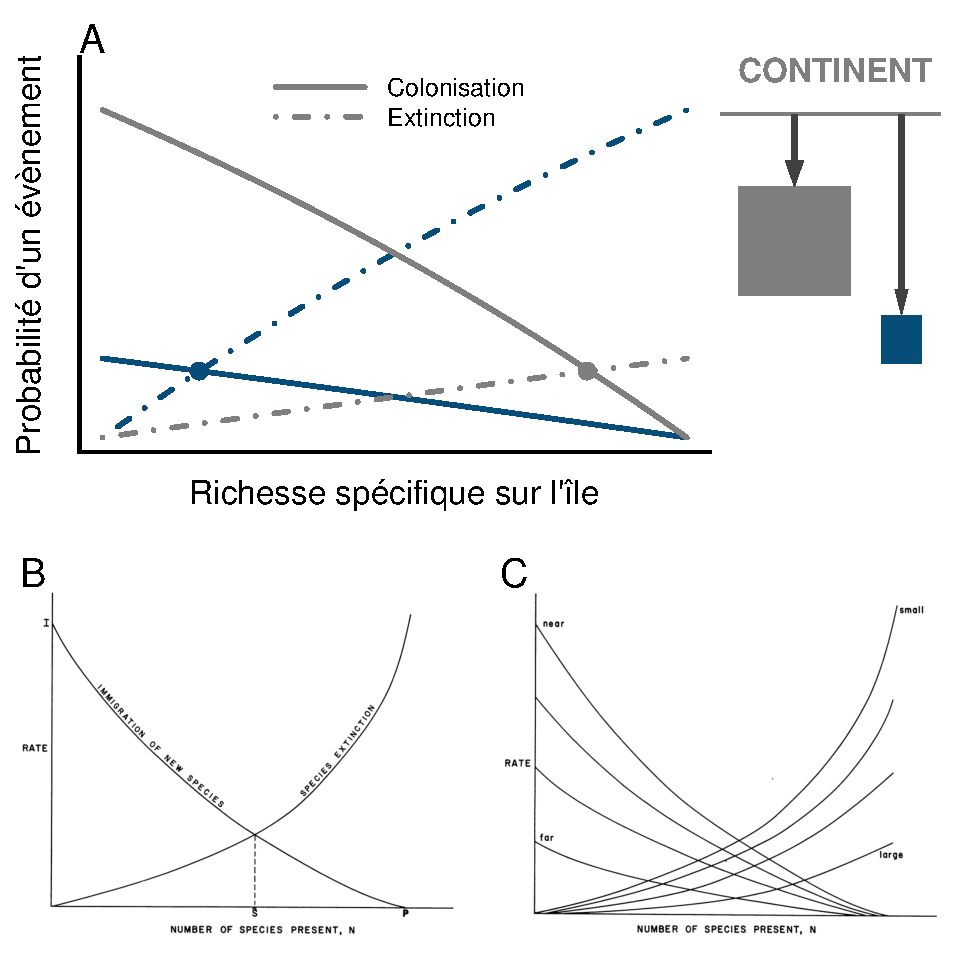
\includegraphics[width=0.80000\textwidth]{fig/fig1.pdf}
\caption{Une tite figfure\label{fig:intr1}}
\end{figure}

Pour faire une ref à la figure \ref{fig:intr1}.

\subsection*{Tables}\label{tables}
\addcontentsline{toc}{subsection}{Tables}

Pour les utilisateur de R, une astuce: faîtes vos tables avec R et
utiliser la fonction `kable' de du package
\href{http://yihui.name/knitr/}{knitr} !!

\begin{longtable}[]{@{}llllrr@{}}
\caption{Une petite légende. \label{tbl:intr_1}}\tabularnewline
\toprule
& Plant & Type & Treatment & conc & uptake\tabularnewline
\midrule
\endfirsthead
\toprule
& Plant & Type & Treatment & conc & uptake\tabularnewline
\midrule
\endhead
8 & Qn2 & Quebec & nonchilled & 95 & 13.6\tabularnewline
16 & Qn3 & Quebec & nonchilled & 175 & 32.4\tabularnewline
24 & Qc1 & Quebec & chilled & 250 & 30.3\tabularnewline
32 & Qc2 & Quebec & chilled & 350 & 38.8\tabularnewline
40 & Qc3 & Quebec & chilled & 500 & 38.9\tabularnewline
48 & Mn1 & Mississippi & nonchilled & 675 & 32.4\tabularnewline
56 & Mn2 & Mississippi & nonchilled & 1000 & 31.5\tabularnewline
64 & Mc1 & Mississippi & chilled & 95 & 10.5\tabularnewline
72 & Mc2 & Mississippi & chilled & 175 & 11.4\tabularnewline
80 & Mc3 & Mississippi & chilled & 250 & 17.9\tabularnewline
\bottomrule
\end{longtable}

Pour faire des référence j'utilise
\href{https://github.com/tomduck/pandoc-tablenos}{pandoc-tablenos} Et
hop je vaos référence à la figured \ref{tbl:intr_1}.

\subsection*{Références
bibliographiques}\label{ruxe9fuxe9rences-bibliographiques}
\addcontentsline{toc}{subsection}{Références bibliographiques}

Pour faire une référence en ligne \citet{Cazelles2016a}; une citation
entre parenthèse \citep{Cazelles2016a}; une citation avec du texte entre
parenthèse \citep[voir][]{Cazelles2016a}. Une succession de citation
\citep{Cazelles2016a, MacArthur1967, DeRuiter1995}.

Références aux autres chapitre. Il faut définir des labels et puis
simplement les appeller en utiisant les \textbackslash{}ref\{chap1\}. Au
chapitre \ref{chap1}, je fais un truc super.

\subsection*{Inclure du code}\label{inclure-du-code}
\addcontentsline{toc}{subsection}{Inclure du code}

Dans une ligne \texttt{x\ \textless{}-\ 3} et pour inclure du code sous
la forme d'un bloc~:

\begin{Shaded}
\begin{Highlighting}[]
\NormalTok{for (i in }\DecValTok{1}\NormalTok{:}\DecValTok{10}\NormalTok{)\{}
  \KeywordTok{print}\NormalTok{(i)}
\NormalTok{\}}
\end{Highlighting}
\end{Shaded}

\begin{Shaded}
\begin{Highlighting}[]
\KeywordTok{for} \KeywordTok{i} \NormalTok{in }\KeywordTok{`seq} \NormalTok{1 6}\KeywordTok{`;} \KeywordTok{do} \KeywordTok{qsub} \NormalTok{start}\OtherTok{$i}\NormalTok{.sh }\KeywordTok{;} \KeywordTok{done}
\end{Highlighting}
\end{Shaded}

